\documentclass[a4paper,11pt, twocolumn]{article}
\usepackage[utf8]{inputenc}
\usepackage{amsmath}
\usepackage{amsfonts}
\usepackage{amssymb}
\usepackage{graphicx}
\usepackage{braket}
\usepackage{sectsty}
\usepackage{biblatex}
\usepackage[font=small]{caption}

\addbibresource{quantum.bib}
\numberwithin{equation}{section}
\renewcommand\thesubsection{\alph{subsection}}
\newcommand{\bvp}[1]{\mathbf{#1}'}
\newcommand{\bv}[1]{\mathbf{#1}}

\sectionfont{\fontsize{10}{10}\selectfont}

%opening
\title{Mechanical coupling of microwave and optical photons}
\author{Vincent Baker, Drexel University Department of Physics}

\begin{document}

\twocolumn[
\begin{@twocolumnfalse}
 \maketitle
 \begin{abstract}
  Quantum electromagnetic phenomenon are of both theoretical and practical interest. 
  Quantum phenomenon are more readily observable at high energies where individual photons are well localized.
  New methods of coherent coupling between optical and microwave systems hold the promise of extending quantum techniques into the microwave regime. 
 \end{abstract}
\end{@twocolumnfalse}
]
\section{Introduction}
Coupling between optical and microwave modes creates a new set of experimental techniques to explore the principles of quantum dynamics.
The coherent transfer of quantum states may be exploited in applications including quantum-enhanced sensing and quantum computing.
Several similar mechanisms for optical/microwave coupling have been reported recently \cite{nanoCrystal, nanoMR}.\\
We will start by reviewing some of the proposed methods for microwave/optical coupling.
We then sketch the analytical exploration of the nanomechanical resonator from \cite{nanoMR} to demonstrate some important aspects of the approach. 
A general discussion of applications is followed by a discussion of aspects of quantum illumination applied to radar systems.

\section{Optical/Microwave Coupling Methods}
Several methods for coupling optical and microwave systems have been investigated. 
In \cite{nanoMR} the authors propose coupling microwave and optical cavity modes through a mechanical resonator.
The resonator itself is a drum-head capacitor that is coupled to the microwave cavity through a planar spiral inductor. 
The equivalent electrical circuit is resonant at microwave frequencies.
One surface of the mechanical resonator is coated with a mirrored finish and caps the end of an optical cavity.
The optically-induced mechanical motion changes the capacitance of the microwave resonator circuit, providing the desired coupling.
\begin{figure}[ht]
 \caption{Optical and microwave cavities entangled through a mechanical resonator. A, Proposed experimental setup. B, Equivalent circuit diagram of microwave resonator.}
 \centering
   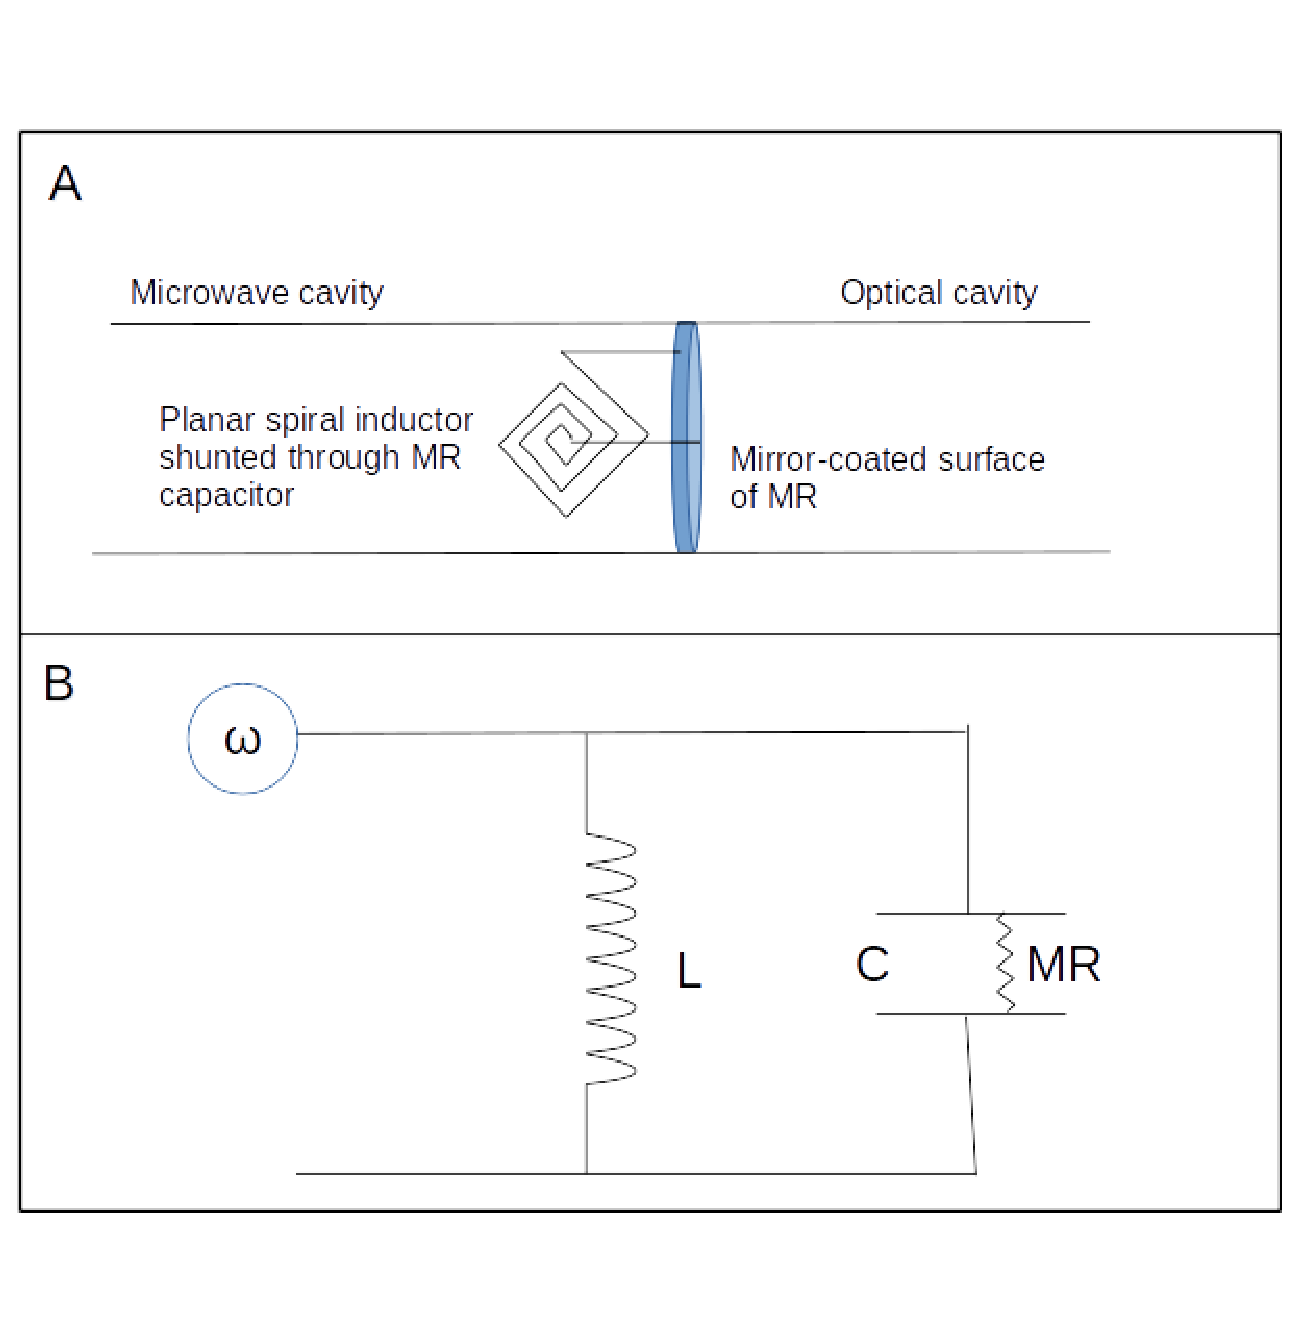
\includegraphics[width=0.5\textwidth]{figs/f1}
\end{figure}
\\In \cite{nanoCrystal} the authors have experimentally characterized a coupled microwave/optical system using a piezoelectric optical nanocrystal.
In this case the nanomechanical coupling function is performed by a piezoelectric optomechanical crystal.
The crystal is driven directly by a microwave signal. 
The optical coupling is acheived by routing an optical waveguide to a separation of <1 optical wavelength from the crystal.
The crystal has a transverse mechanical resonance at 4GHz which is electrically excited.
The optical coupling point (see figure \ref{fig:optoCrystal}) is placed at the mechanical resonance point, so that the electrically excited mechanical motion interacts with the optical transmission.
\begin{figure}[ht]
 \caption{Optomechanical piezo crystal device from \cite{nanoCrystal}.}
 \centering
   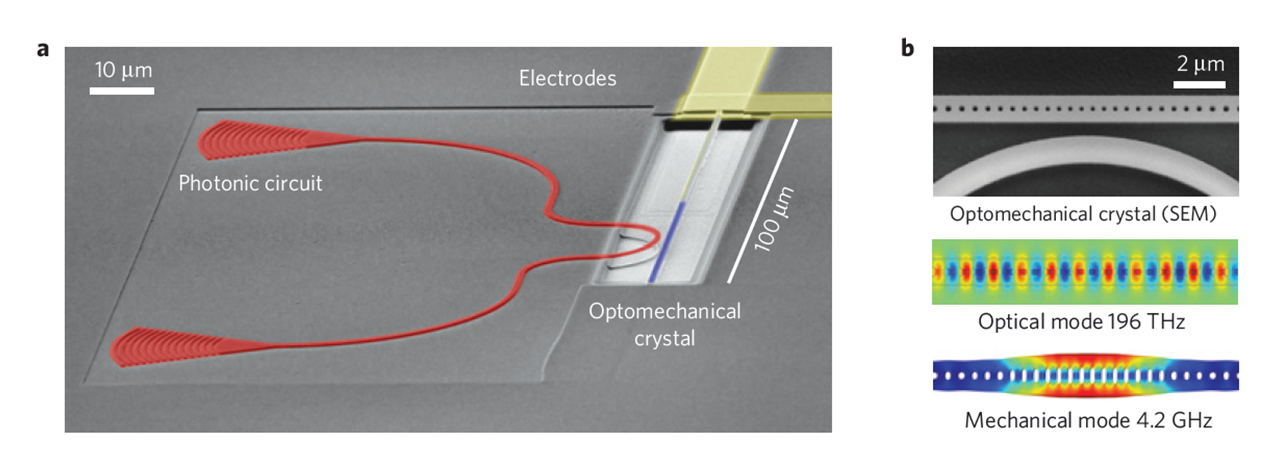
\includegraphics[width=0.5\textwidth]{figs/OptoMechCrystal}
 \label{fig:optoCrystal}
\end{figure}
\\
The authors in \cite{nanoCrystal} focus on the ability to transfer phase and amplitude from the microwave signal to the optical signal.
Figure \ref{fig:homodyne} shows the experimental setup using homodyne mixing of an optical signal that has been downcoverted through photodetection and low-pass filtering to isolate the optical sideband related to the mechanical resonance.
The Argand diagram of the received signal for different phases of the injected microwave signal show that the microwave phase is retained in the coupled optical signal.
\begin{figure}[ht]
 \caption{Homodyne detection from \cite{nanoCrystal}.}
 \centering
   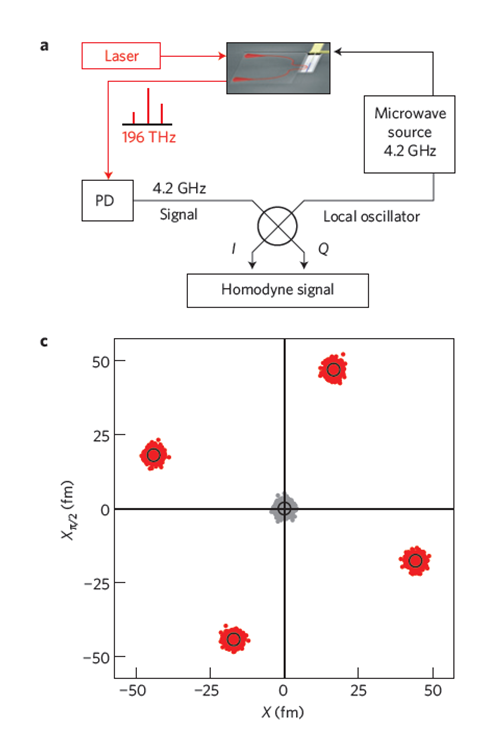
\includegraphics[width=0.5\textwidth]{figs/CrystalMixing}
 \label{fig:homodyne}
\end{figure}
\\
The optomechanical piezoelectric crystal was fabricated as an integrated electronic/photonic device.
This is a strongly supported area of engineering research, as exemplified by the new Integrated Photonics Institute for Manufacturing Innovation, 
an institute with almost 100 academic and industry members funded with \$110M federal funding and over \$500M cost share from the members \cite{ipimi}.
As these engineering and manufacturing methods improve these types of nanomechanical systems will become readily available to physics researchers.

\section{Analysis of the Mechanical Resonator Dynamics}
We present the analysis of the nanomechanical resonator system in \cite{nanoMR} to illustrate some of the relevant analytical methods.
The Hamiltonian of the combined system is expressed in terms of the creation and annihilation operators of the optical and microwave cavities.
The effects of thermal noise are incorporated through a set of quantum Langevin equations, which are then linearized about a stationary point. 
Finally the correlation matrix of the system is developed, from the which the logarithmic negativity can be calculated.
The log-negativity is a measure of the degree of entanglement between the elements of the system, and the results demonstrate the entanglement between the optical and microwave modes.
\\
We treat the nanomechanical resonator as a one-dimensional harmonic oscillator. 
We use the subscripts $w,m,c$ to denote parameters of the microwave cavity, mechanical resonator and optical cavity respectively.
The cavities are driven at frequencies detuned from resonance by $\Delta_{0w}$ and $\Delta{0c}$.
The Hamiltonian of the system shown in figure 1 is then:
\begin{align}
\begin{split}
 H = &\frac{p_x^2}{2m}+\frac{m\omega_m^2x^2}{2}\\
     &+\frac{\Phi^2}{2L}+\frac{Q^2}{2(C+C_0(x))}-e(t)Q\\
     &+\hbar\omega_c a^\dagger a-\hbar G_{0c}a^\dagger ax\\
     &+i\hbar E_c\left(a^\dagger e^{-i\omega_{0c}t}-ae^{i\omega_{0c}t} \right)
 \end{split}
\end{align}
Where $a^\dagger,a$ are the creation and annihilation operators of the optical cavity, $\Phi,Q$ are the flux through the inductor and the charge on the capacitor,
$e(t)=-i\sqrt{2\hbar\omega_wL}E_w\left(e^{i\omega_{0w}t}-e^{-i\omega_{0w}t} \right)$ is the driving function of the microwave cavity
and $G_{0c}\frac{\omega_c}{L}\sqrt{\hbar/m\omega_m} $ gives the optomechanical coupling rate with resonator mass m and optical cavity length L.
\\
The quadratic form of the microwave resonator circuit is amenable to expression in terms of microwave creation and annihilation operators $b,b^\dagger$.
We can then work in the interaction picture with respect to:
\begin{align}
 H_0 &= \hbar\omega_{0w}b^\dagger b +\hbar\omega_{0c}a^\dagger a
\end{align}
We can now express the time-dependent Hamiltonian in terms of the cavity detunings and neglect higher-order terms at $\pm2\omega_{0w},\pm2\pm\omega_{0c}$ since they will oscillate quickly and tend to average out.
The final Hamiltonian is:
\begin{align}
\begin{split}
 H = &\hbar\Delta_{0w}b^\dagger b+\hbar\Delta_{0c}a^\dagger a\\
     &+\frac{\hbar\omega_m}{2}(\hat{p}^2+\hat{q}^2)-\hbar G_{0w}\hat{q}b^\dagger b-\hbar G_{0c}\hat{q}a^\dagger a\\
     &+i\hbar E_w(b^\dagger -b)+i\hbar E_c(a^\dagger -a )
\end{split}
\end{align}
The fourth and fifth terms of the Hamiltonian are the coupling terms between the microwave and optical cavities and the mechanical resonator.\\ 
We also consider thermal effects for both systems. We plot the expected number of thermal photons for both the optical system (500 THz) and the microwave system (4.5 GHz) in Figure \ref{fig:thermalnoise}.
\begin{align}
 \braket{n}_e &= \frac{1}{z^{-1}e^{\beta \hbar \omega}-1}
\end{align}
\begin{figure}[ht]
 \caption{Mean number of thermal photons in the microwave cavity (top) and the optical cavity (bottom)}
 \centering
   \includegraphics[width=0.5\textwidth]{figs/ThermalPhotons}
 \label{fig:thermalnoise}
\end{figure}
We can clearly neglect thermal noise in the optical part of the system, but we must include noise terms in the microwave system even at low temperatures.
To incorporate the noise terms the authors introduce a set of quantum Langevin equations (QLEs), differential equations for the time evolution of the system.
\begin{align}
 \dot{q} &= \omega_mp\\
 \dot{p} &- -\omega_mq-\gamma_mp+G_{0c}a^\dagger a+G_{0w}b^\dagger b +\xi\\
 \dot{a} &= -(\kappa_c+i\Delta_{0c})a+iG_{0c}qa+E_c\\
 \begin{split}
 \dot{b} &= -(\kappa_w+i\Delta_{0w})b+iG_{0w}qb+E_w\\
         &\ \ +\sqrt{2\kappa_w}b_{in}
 \end{split}
\end{align}
Where $\kappa_c,\kappa_w$ are the damping functions of the optical and microwave cavities, $\xi$ is the quantum Brownian noise acting on the mechanical resonator,
and $b_{in}$ is the noise function for the microwave input.\\
The authors then investigate the steady state of the driven system by setting the derivatives in the QLEs equal to 0. 
One question not addressed in this paper is the time for the system to reach steady state. 
This settling time will be important for quantum illumination systems that use pulsed signals that are not continuous in time.
The authors  write the steady-state parameter values as $q_s,p_s,a_s, b_s$ with corresponding fluctuations $\delta q,\delta p,\delta a,\delta b$.
The equilibrium values are found by setting the derivatives to 0:
\begin{align}
 p_s &= 0\\
 q_s &= \frac{G_{0c}|a_s|^2+G_{0w}|b_s|^2}{\omega_m}\\
 a_s &= \frac{E_c}{\kappa_c+i\Delta_c}\\
 b_s &= \frac{E_w}{\kappa_w+i\Delta_w}
\end{align}
Where we have written $\Delta_c=\Delta_{0c}-G_{0c}q_s$ and $\Delta_w=\Delta_{0w}-G_{0w}q_s$. 
These are the caivty detunings for the optical and microwave fields. 
Expanding about the equilibrium point:
\begin{align}
 \delta\dot{q} &= \omega_m\delta p\\
 \begin{split}
 \delta\dot{p} &= -\omega_m\delta q -\gamma_m\delta p +G_{0c}a_s(\delta a^\dagger+\delta a)\\
               &\ +G_{0w}b_s(\delta b^\dagger+\delta b)+\xi
 \end{split}\\
 \delta\dot{a} &= -(\kappa_c+i\Delta_c)\delta a + iG_{0c}a_s\delta q + \sqrt{2\kappa_c}a_{in}\\
 \delta\dot{b} &= -(\kappa_w+i\Delta_w)\delta b + iG_{0w}b_s\delta q
\end{align}
Having obtained the dynamics of the fluctuations of the system about the equilibirum point, the authors now analyze the correlations between the three component systems.

\section{Correlation analysis}
There are several measures of entanglement in quantum information theory. 
A bipartite system is completely separable (unentangled) if it can be written as combinations of the tensor product of the component systems:
\begin{align}
 \rho^{ab} &= \sum_i c_i \rho_i^a \otimes \rho_i^b
\end{align}
When $\rho^{ab}$ is a pure state the degree of entanglement can be determined from reduced density matrix with respect to one of the component systems:
\begin{align}
 \rho^a \equiv Tr_b(\rho^{ab} )\\
 S = -Tr(\rho^a\ln{\rho^a} )
\end{align}
For mixed states the evaluation is more complicated. 
In \cite{qent} the authors introduce a computable entanglement metric for a bipartite mixed state, the negativity:
\begin{align}
 N(\rho) \equiv \frac{\|\rho^{T_a}\|_1}{2}
\end{align}
Where $\|\rho^{T_a}\|_1$ is the trace norm of the partial transpose of $\rho$ with respect to component system a.

\section{Discussion of quantum radar}
Quantum-enhanced sensing is a relatively young field that seeks to enhance sensing by using quantum entanglement. 
We discuss the particular application of quantum illumination in the microwave regime applied to radar systems.
Radar systems determine the range, bearing and velocity of an object by emitting a microwave signal and measuring the signal reflections.
Radar waveforms are designed to allow the receiver to correlate the return signal from an object of interest in the presence of thermal noise, interfering signals and signal reflections from other objects.
Quantum illumination can improve this correlation and can theoretically provide better performance than any conventional microwave system \cite{qi}(other MIT citations).
\\
In microwave quantum illumination the microwave probe photon will travel from the transmitter to the object to be detected, scatter from the object, and return to the detector.
An optical photon, termed the idler photon, is initially entangled with the microwave photon (figure \ref{fig:quantumradar}).
The probe photons are not expected to remain in a coherent entangled state with the idler photons, yet there is a still an enhanced correlation between them even after decoherence \cite{qig}. 
\begin{figure}[ht]
 \caption{Quantum radar conceptual design from \cite{qi}}
 \centering
   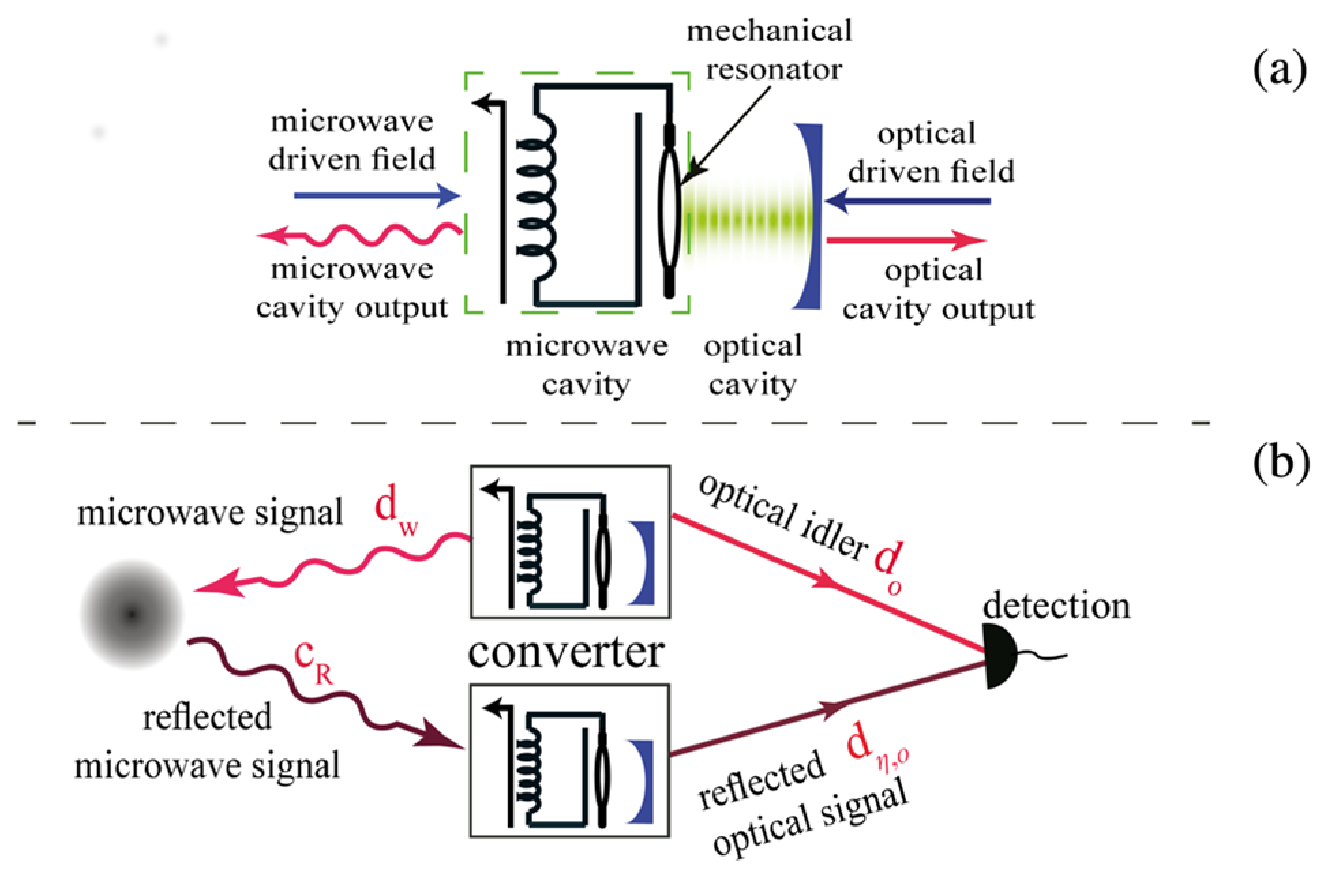
\includegraphics[width=0.5\textwidth]{figs/QuantumRadar}
 \label{fig:quantumradar}
\end{figure}
\\
The key result \cite{qig} was to compare theorectical bounds on detection performance between a quantum illumination system and a coherent system.
The authors analyzed an optical quantum illuminator detecting a weak scatterer in a strong thermal bath, so that there were many more thermal noise photons than scattered photons received at the detector. 
As shown in figure 2 this is an artifical situation as thermal effects are generally negligble at optical energies.
The authors in \cite{qi} present microwave quantum illumination as a more realistic application of the same principles.
\\
Even in the microwave regime the results in \cite{qig} and \cite{qi} are not necessarily relevant. 
Radar systems can employ very high-power microwave sources and highly directional antennas.
Radar system performance is in general not limited by the thermal background noise but instead by ``clutter'': the scattered radar signals from objects not of interest.
Typical clutter scatterers include ground, foliage, buildings, rain and other atmospheric particulate.
Moder radar systems mitigate clutter effects through the use of short signal pulses, directional antennas, and sophisticated waveforms.
Any radar system employing quantum illumination must be able to employ similar techniques, or else the gains from quantum coherence will be more than offset by other losses. 
\\
Modern radar designs are dominated by the electronically steered array (ESA) antenna. 
An electronically steered antenna consists of many individual antenna elements, with each element able to individually control the phase shift of the transmitted and received signal.
Two types of ESA are shown in figure \ref{fig:phasedarrays}. The passive ESA in the top figure has a single high-power microwave source, which illuminates a planar array of antenna elements.
Each element in the array includes an electronically controlled phase shifter that changes the phase of the signal as it passes through.
The lower figure shows an active ESA in which every antenna element includes a separate microwave source.
\begin{figure}[ht]
 \caption{Passive (top) and active (bottom) phase arrays. In the active array, each element has a microwave source.}
 \centering
   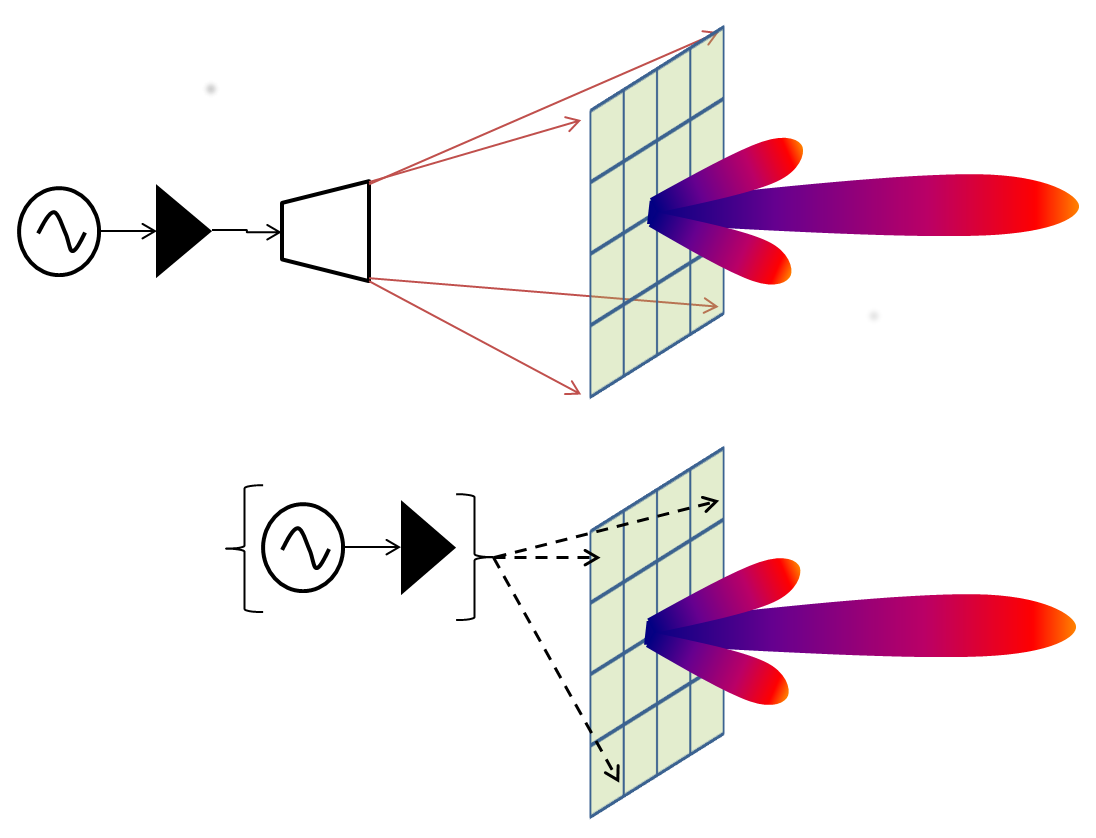
\includegraphics[width=0.5\textwidth]{figs/PhasedArrays}
 \label{fig:phasedarrays}
\end{figure}
\\
Applying quantum illumination to a phased array system will require the resolution of several questions.
The schemes discussed so far may be compatible with a passive ESA. but it must be determined if passing the signal through many passive phase shifters will degrade the correlation with the idler signal.
It is not alear how quantum illumination would be applied to an active ESA design. The active ESA signals are digitized at each individual element, and the antenna beamforming and signal correlation is done in the digital domain.


\printbibliography
\end{document}
